\clearpage		\large
\chapter{Test Fixture Drawings} \label{App:test_figure_drawings}

\begin{table}[H]
\centering
\begin{tabular}{|L{0.23\textwidth}|C{0.08\textwidth}|C{0.08\textwidth}|C{0.08\textwidth}|C{0.08\textwidth}|L{0.25\textwidth}|}
\hline
Item 								&Length (in) 	&Width (in) 	&Height (in) 	&Weight (lbs.) 	&Material \\ \hline \hline
King Mattress 						&79.0 			&71.0 			&10.0 			&76.0 			&52\% Polyurethane Foam, 30\%, Blended Cotton Batting, \& 18\% Polyester Fiber Batting \\ \hline
King Box Spring 					&78.0 			&35.0 			&7.0			&46.0 			&59\% Fiber Pad, 41\% Blended Cotton Batting \& Wood Frame \\ \hline
King Headboard 						&78.0			&24.0 			&1.0			&54.0 			&Medium Density Fiberboard \\ \hline
Pillow 								&23.5 			&17.0 			&4.0			&1.5 			&Filling - All Polyester, Cover - 100\% Cotton \\ \hline
Comforter 							&104.0 			&92.0 			&1.0			&4.6 			&Cover - 100\% Polyester, Fill - 100\% Polyester \\ \hline
Mattress Topper 4 in 				&78.0 			&75.0 			&3.9 			&16.0  			&Viscoelastic Polyurethane Foam Pad 100\% \\ \hline
Night Stand 						&18.0 			&27.0 			&23.4	 		&60.0 			&Solid Wood \\ \hline
Dresser 							&22.1	 		&36.0 			&34.25 			&120.0 			&Wood \& Plywood \\ \hline
Curtain (Small) 					&39.0 			&73.0 			&0.1 			&4.5 			&Flame Retardant \& Synthetic Fibers \\ \hline
Sofa Chair (Yellow/Green) 			&31.3 			&31.0 			&39.0 			&54.0 			&Polyester Fiber 75\%, Polyurethane Foam 25\%, Pillow - Polyurethane Foam 90\%, Polyester Batting 10\% \\ \hline
Sofa Chair (Red Lines) 				&34.5 			&34.0 			&32.0 			&63.0 			&Urethane Foam 100\% \\ \hline
Sofa Chair (Red Swirl) 				&34.0 			&34.0 			&32.0 			&70.0 			&Blended Cotton Felt 100\%, Cushion, Polyurethane Foam 100\% \\ \hline
Sofa Chair (Red Diamond) 			&35.0 			&35.0 			&34.0 			&69.0 			&Polyurethane Foam (Blended Cotton or, Polyester when used is less than 10\%) \\ \hline
\end{tabular}
\caption{Bedroom Fuel Load Information}
\label{table:bd_fuel_weights}
\end{table}

\begin{table}[H]
\centering
\begin{tabular}{|L{0.23\textwidth}|C{0.08\textwidth}|C{0.08\textwidth}|C{0.08\textwidth}|C{0.08\textwidth}|L{0.25\textwidth}|}
\hline
Item 								&Length (in) 	&Width (in) 	&Height (in) 	&Weight (lbs.) 	&Material \\ \hline \hline
Curtain (Large) 					&107.0 			&73.0 			&0.1 			&13.7 			&Flame Retardant \& Synthetic Fibers \\ \hline
Mattress Topper 5 in 				&77.5 			&76.3 			&4.6 			&20.1  			&Urethane Foam \\ \hline
Kitchen Table 						&52.0 			&26.0 			&24.5 			&29.1 			&Particleboard \& Wood \\ \hline
Straight Chair (Pink) 				&18.0 			&19.0 			&33.0 			&15.2 			&Wood \& Upholstery \\ \hline
Straight Chair (Blue) 				&19.0 			&19.0 			&38.9			&14.9 			&Wood \& Upholstery \\ \hline
Bookcase 							&11.5 			&24.6	 		&71.3 			&46.0 			&Particleboard \\ \hline
TV Stand 							&22.1	 		&36.0 			&34.3 			&120.0 			&Wood \& Plywood \\ \hline
Sofa 								&35.0 			&77.0 			&30.5 			&255.0 			&Polyurethane Foam 50\%, Polyester Fiber 50\%,\& Wood Frame \\ \hline
Sofa Chair (Striped) 				&33.0 			&35.0 			&33.5 			&65.0 			&Polyurethane Foam 75\% Polyester Fiber 25\% \\ \hline
Ottoman 							&19.8 			&25.5 			&16.0 			&21.3 			&Upholstery \\ \hline
Coffee Table 			 			&30.0 			&18.0 			&18.3 			&24.4 			&Particleboard \& Wood \\ \hline
End Table 			 				&24.3 			&24.3 			&22.1	 		&32.1 			&Solid Wood \\ \hline
Table Lamp Base 					&5.8 			&5.3 			&31.3 			&5.9 			&Glass, Metal  \\ \hline
Table Lame Shade 					&14.4	 		&14.4	 		&  				&  				&Cloth Shade \\ \hline 
\end{tabular}
\caption{Kitchen and Living Room Fuel Load Information}
\label{table:k_lv_fuel_weights}
\end{table}

\begin{table}[H]
\centering
\begin{tabular}{|L{0.23\textwidth}|C{0.08\textwidth}|C{0.08\textwidth}|C{0.08\textwidth}|C{0.08\textwidth}|L{0.25\textwidth}|}
\hline
Item 								&Length (in) 	&Width (in) 	&Height (in) 	&Weight (lbs.) 	&Material \\ \hline \hline
Bedroom 1 Carpet (Room) 			&13.3			&12.8			&0.4			&47.6			&Polyester 100\% \\ \hline
Bedroom 1 Carpet (Closet)			&7.5			&2.9			&0.4			&6.0			&Polyester 100\% \\ \hline
Bedroom 1 Carpet Padding (Room)		&13.3			&12.8			&				&27.2			& \\ \hline
Bedroom 1 Carpet Padding (Closet)	&7.5			&2.9			&				&3.4			& \\ \hline	 	 
Bedroom 2 Carpet (Room) 			&11.0			&12.8			&0.4			&39.3			&Polyester 100\% \\ \hline
Bedroom 2 Carpet (Closet)			&6.1			&1.9			&0.4			&3.2			&Polyester 100\% \\ \hline
Bedroom 2 Carpet Padding (Room)		&11.0			&12.8			&				&22.4			& \\ \hline
Bedroom 2 Carpet Padding (Closet)	&6.1			&1.9			&				&1.8			& \\ \hline	  
Bedroom 3 Carpet 					&11.0			&12.8			&0.4			&39.3			&Polyester 100\% \\ \hline
Bedroom 3 Carpet Padding 			&11.0			&12.8			&				&22.4			& \\ \hline	 
Bedroom 4 Carpet 					&11.1			&12.8			&0.4			&39.6			&Polyester 100\% \\ \hline
Bedroom 4 Carpet Padding 			&11.1			&12.8			&				&22.6			& \\ \hline	 
Kitchen Carpet 						&12.8			&18.8			&0.4			&67.1			&Polyester 100\% \\ \hline
Kitchen Carpet Padding 				&12.8			&18.8			&				&38.3			& \\ \hline	 
Living Room Carpet					&16.1			&19.1			&0.4			&85.5			&Polyester 100\% \\ \hline 
Living Room Carpet Padding 			&16.1			&19.1			&				&49.5			& \\ \hline	
\end{tabular}
\caption{Carpet and Padding Fuel Load Information}
\label{table:carpet_padding_fuel_weights}
\end{table}

\begin{sidewaysfigure}
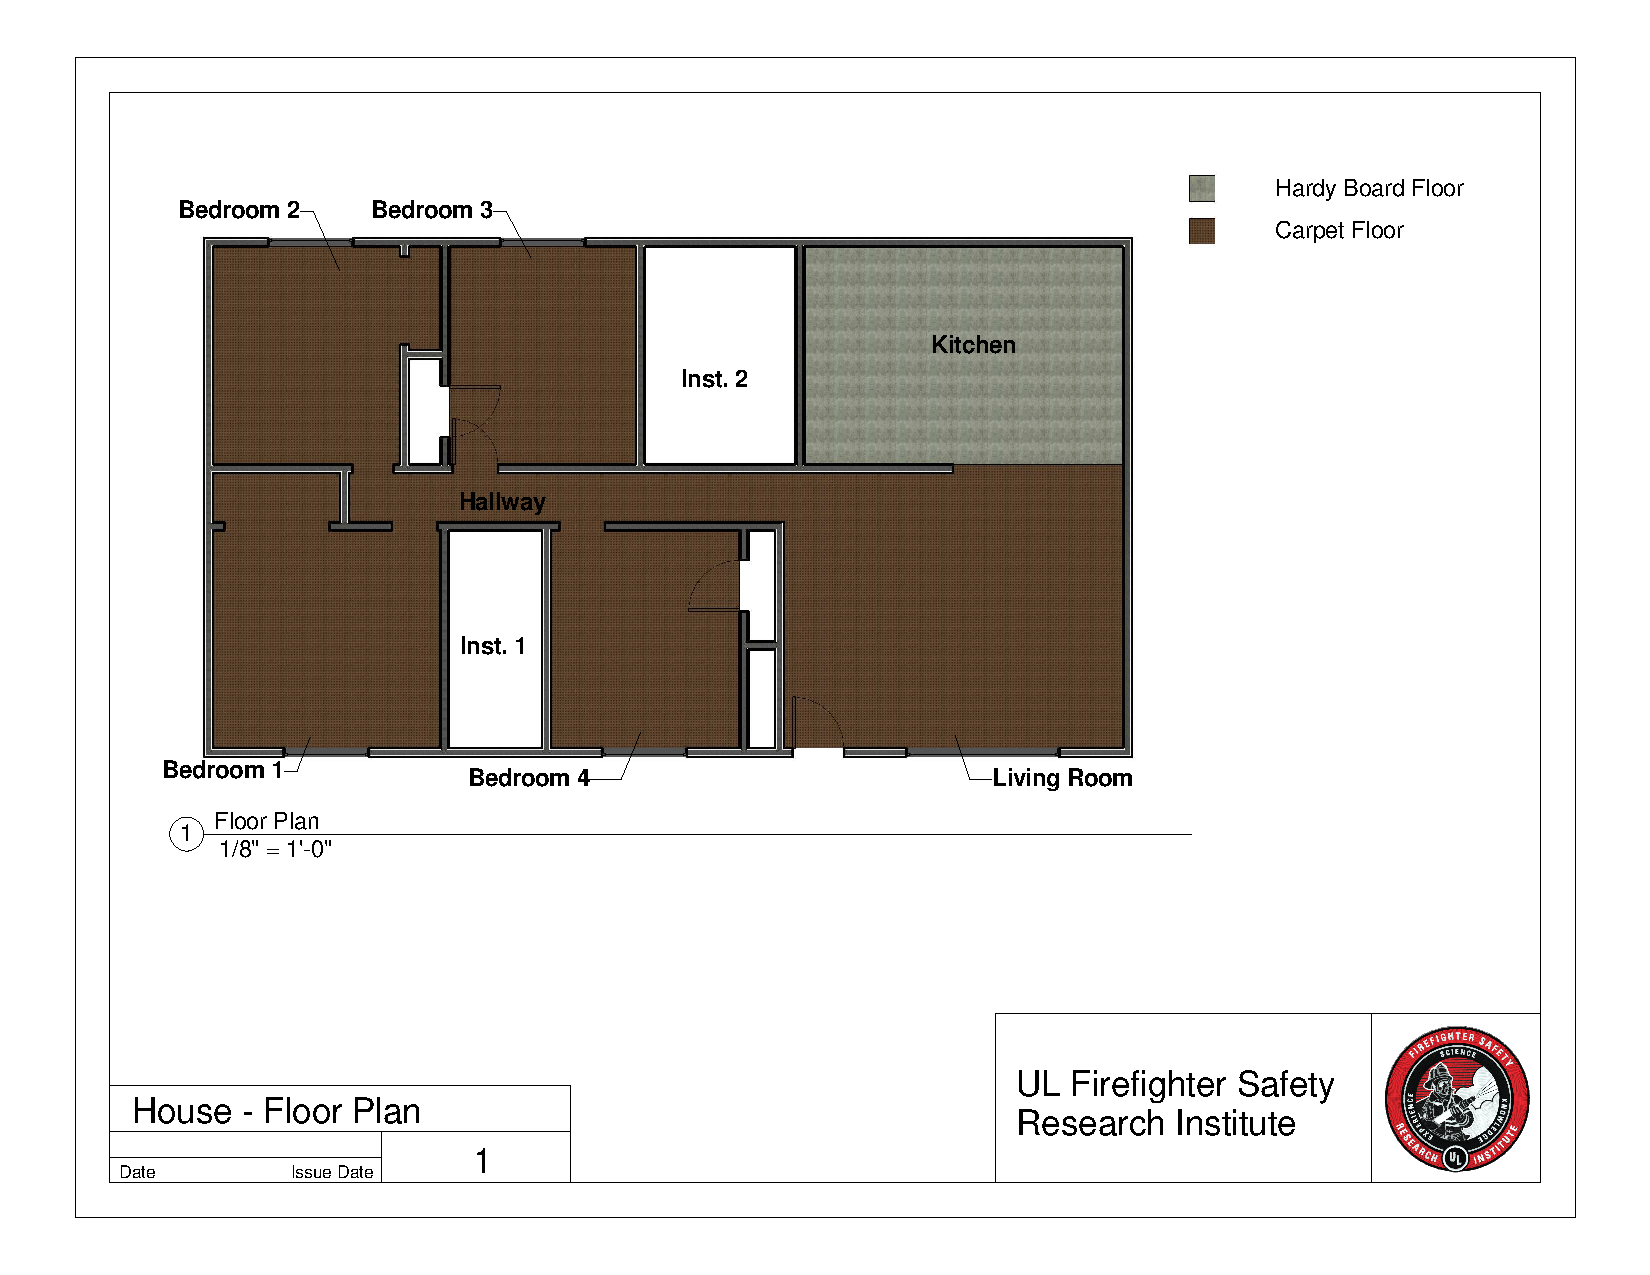
\includegraphics[width=\textheight]{../0_Images/Appendix_Figures/Floor_Plan}
\caption[]{Test Fixture Floor Plan}
\label{fig:appendix_floorplan}
\end{sidewaysfigure}

\begin{sidewaysfigure}
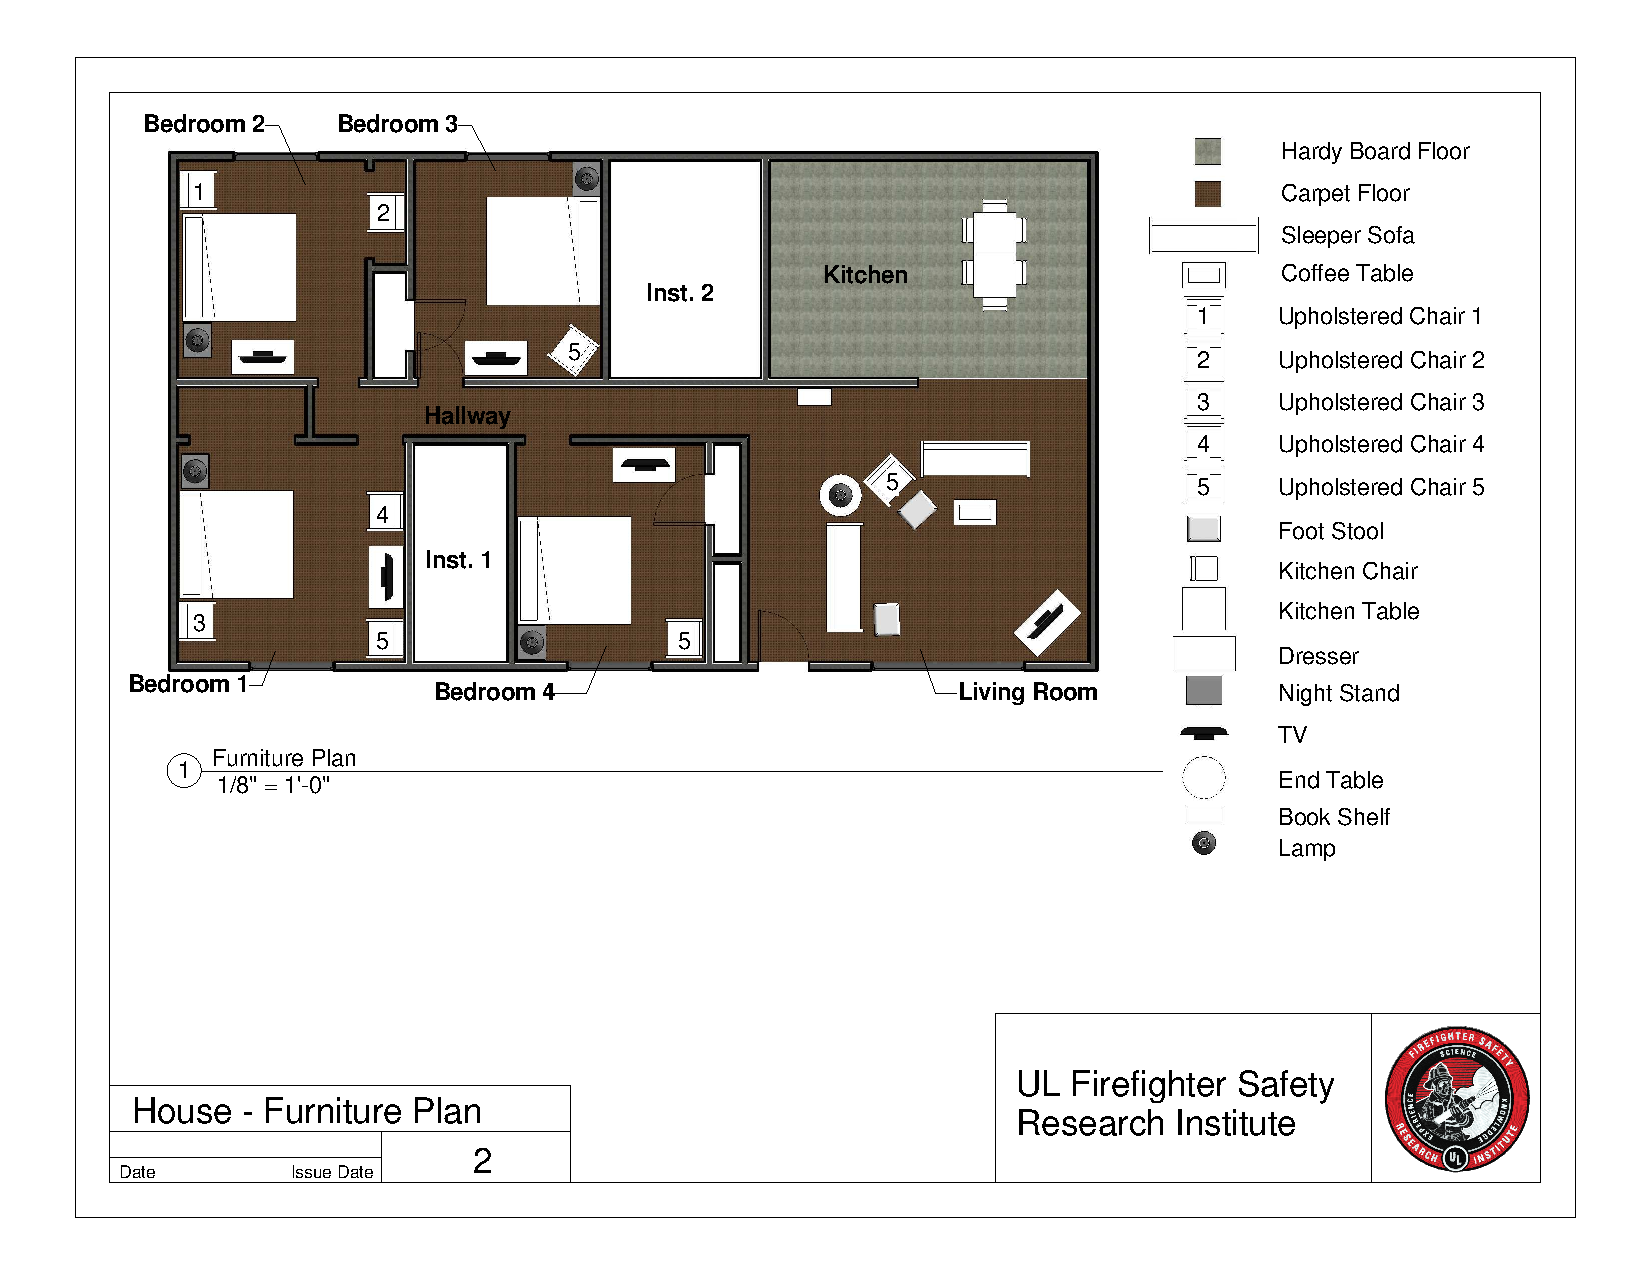
\includegraphics[width=\textheight]{../0_Images/Appendix_Figures/Furniture_Plan}
\caption[]{Test Fixture Furniture Plan}
\label{fig:appendix_furnitureplan}
\end{sidewaysfigure}

\begin{sidewaysfigure}
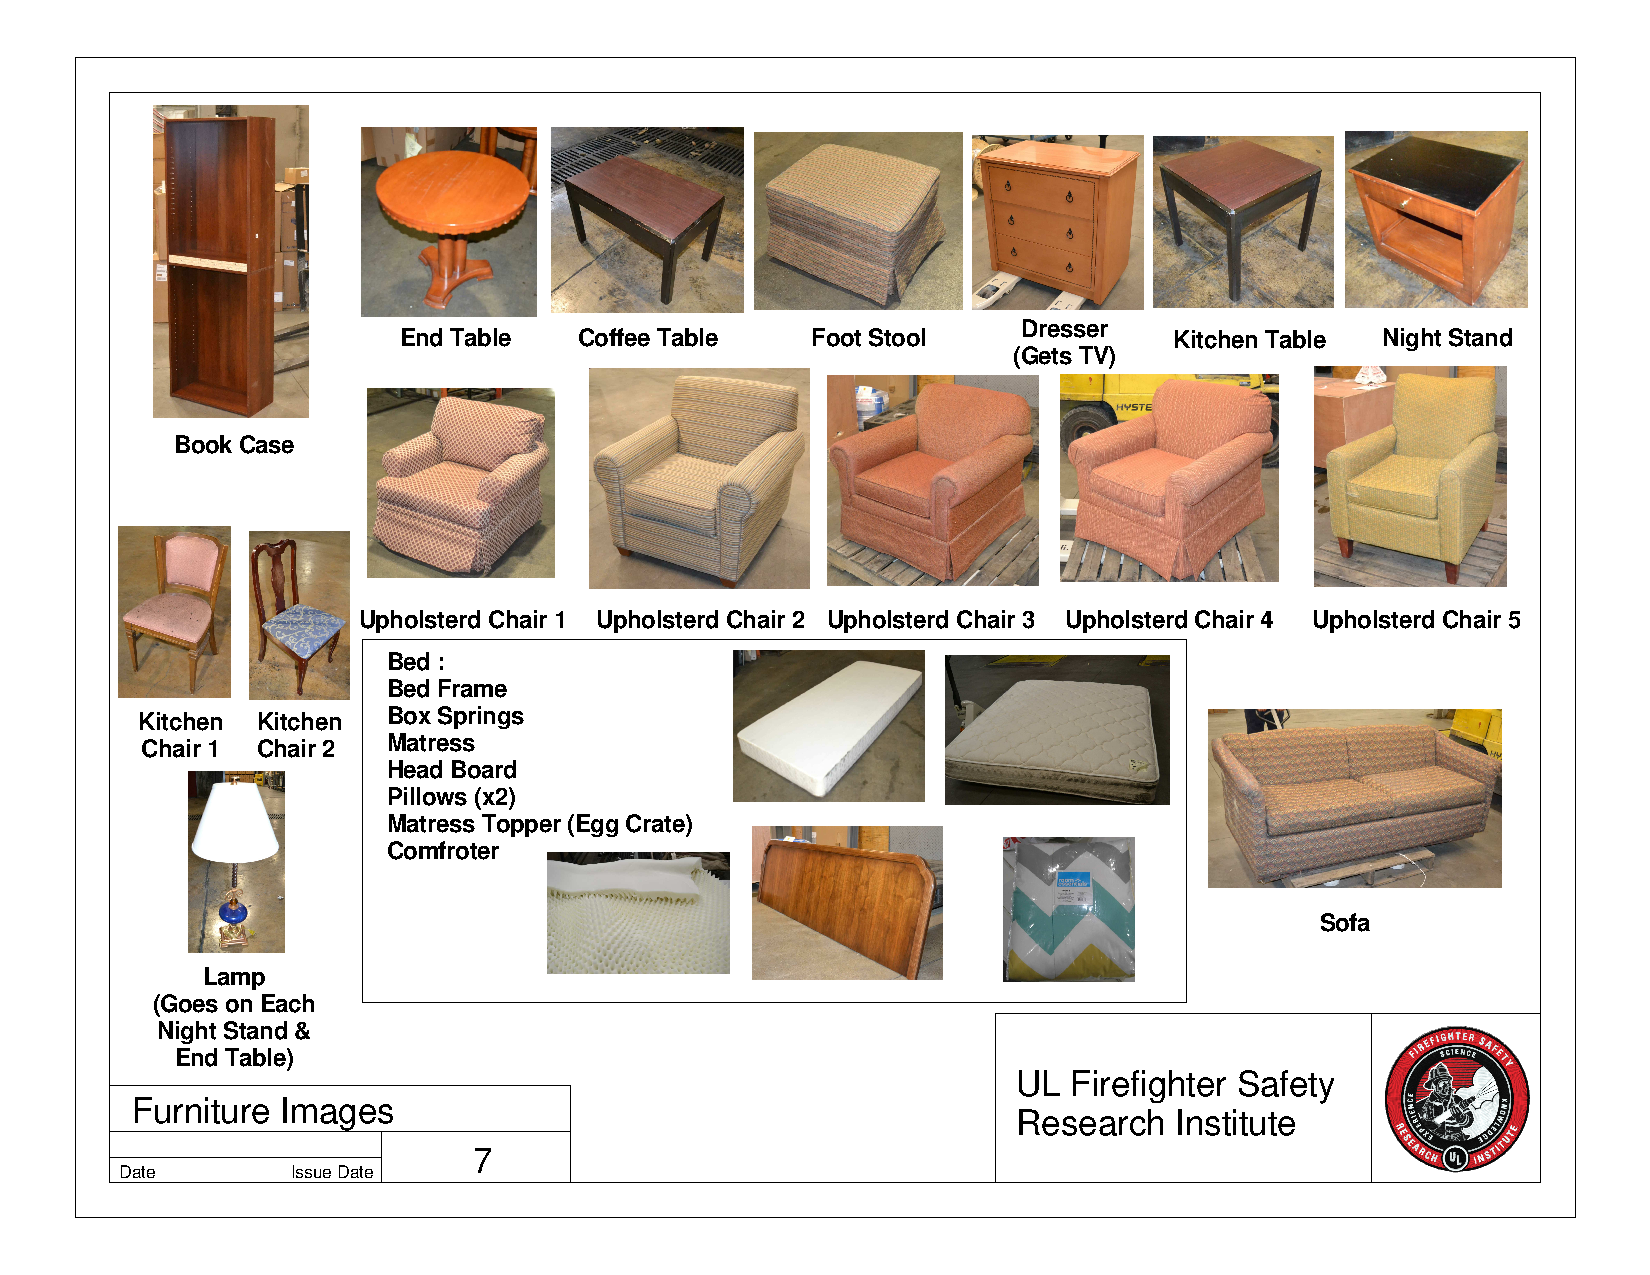
\includegraphics[width=\textheight]{../0_Images/Appendix_Figures/Furniture_Images}
\caption[]{Test Fixture Furniture Images}
\label{fig:appendix_furnitureimages}
\end{sidewaysfigure}

\begin{sidewaysfigure}
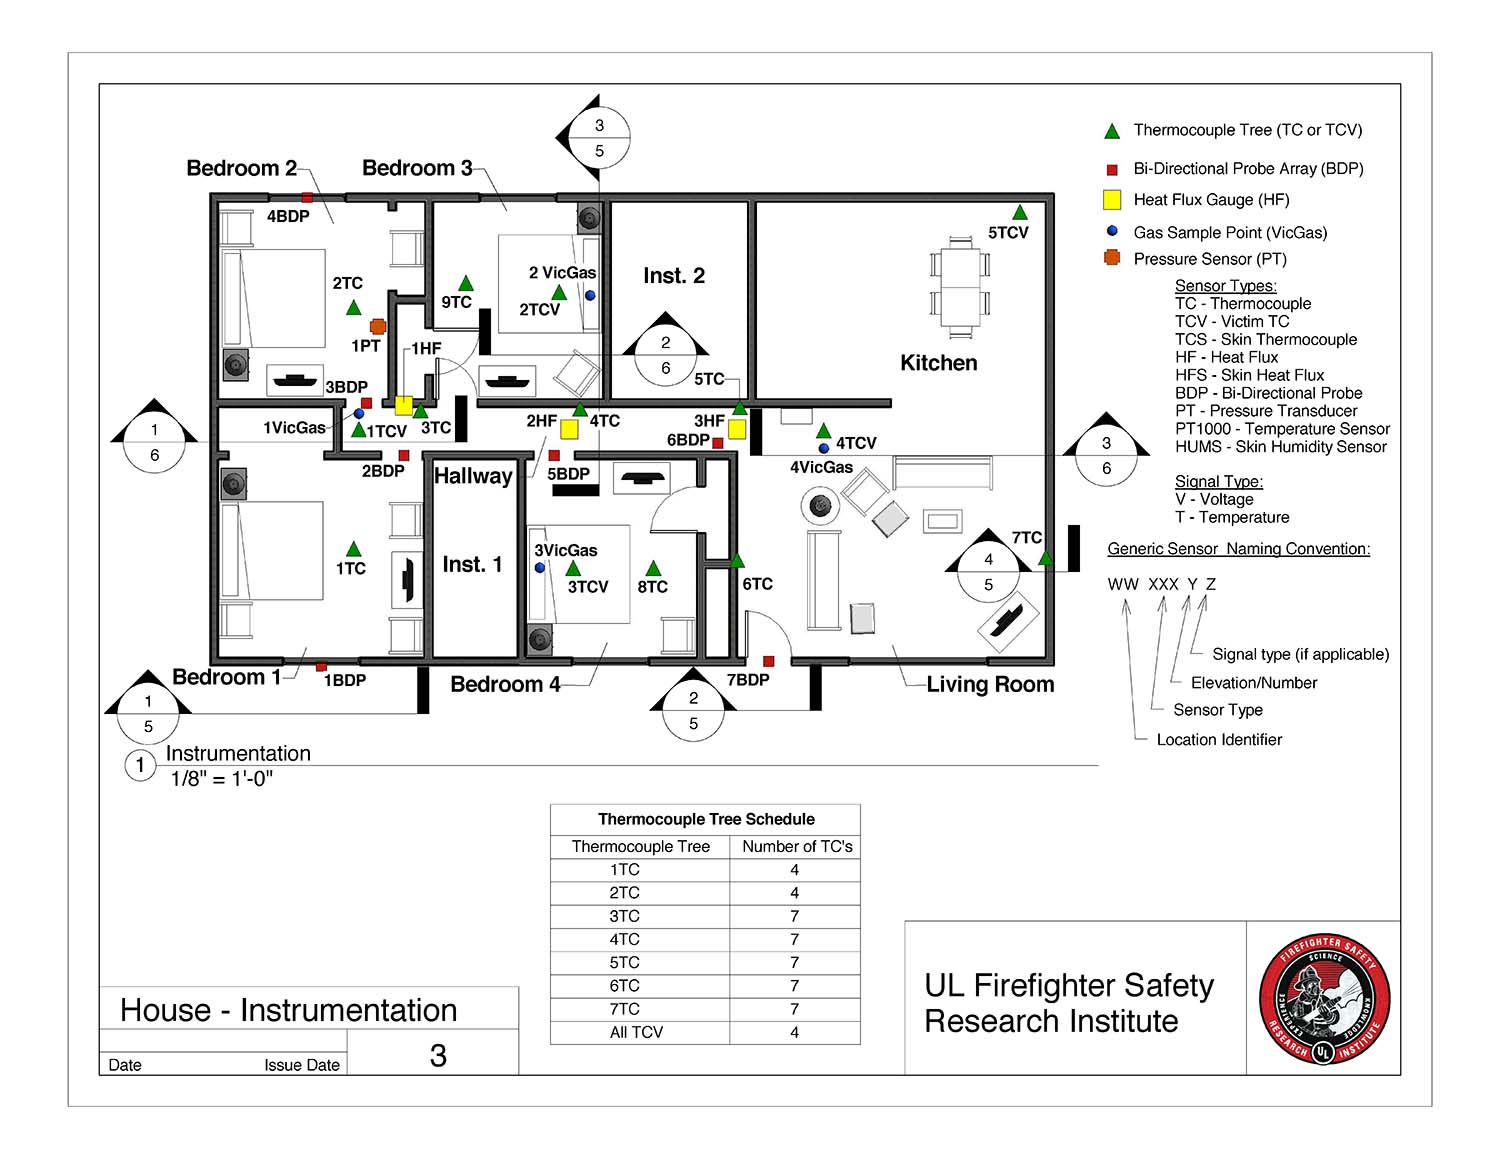
\includegraphics[width=\textheight]{../0_Images/Appendix_Figures/Instrument_Plan}
\caption[]{Instrumentation Plan}
\label{fig:appendix_instruments}
\end{sidewaysfigure}

\begin{sidewaysfigure}
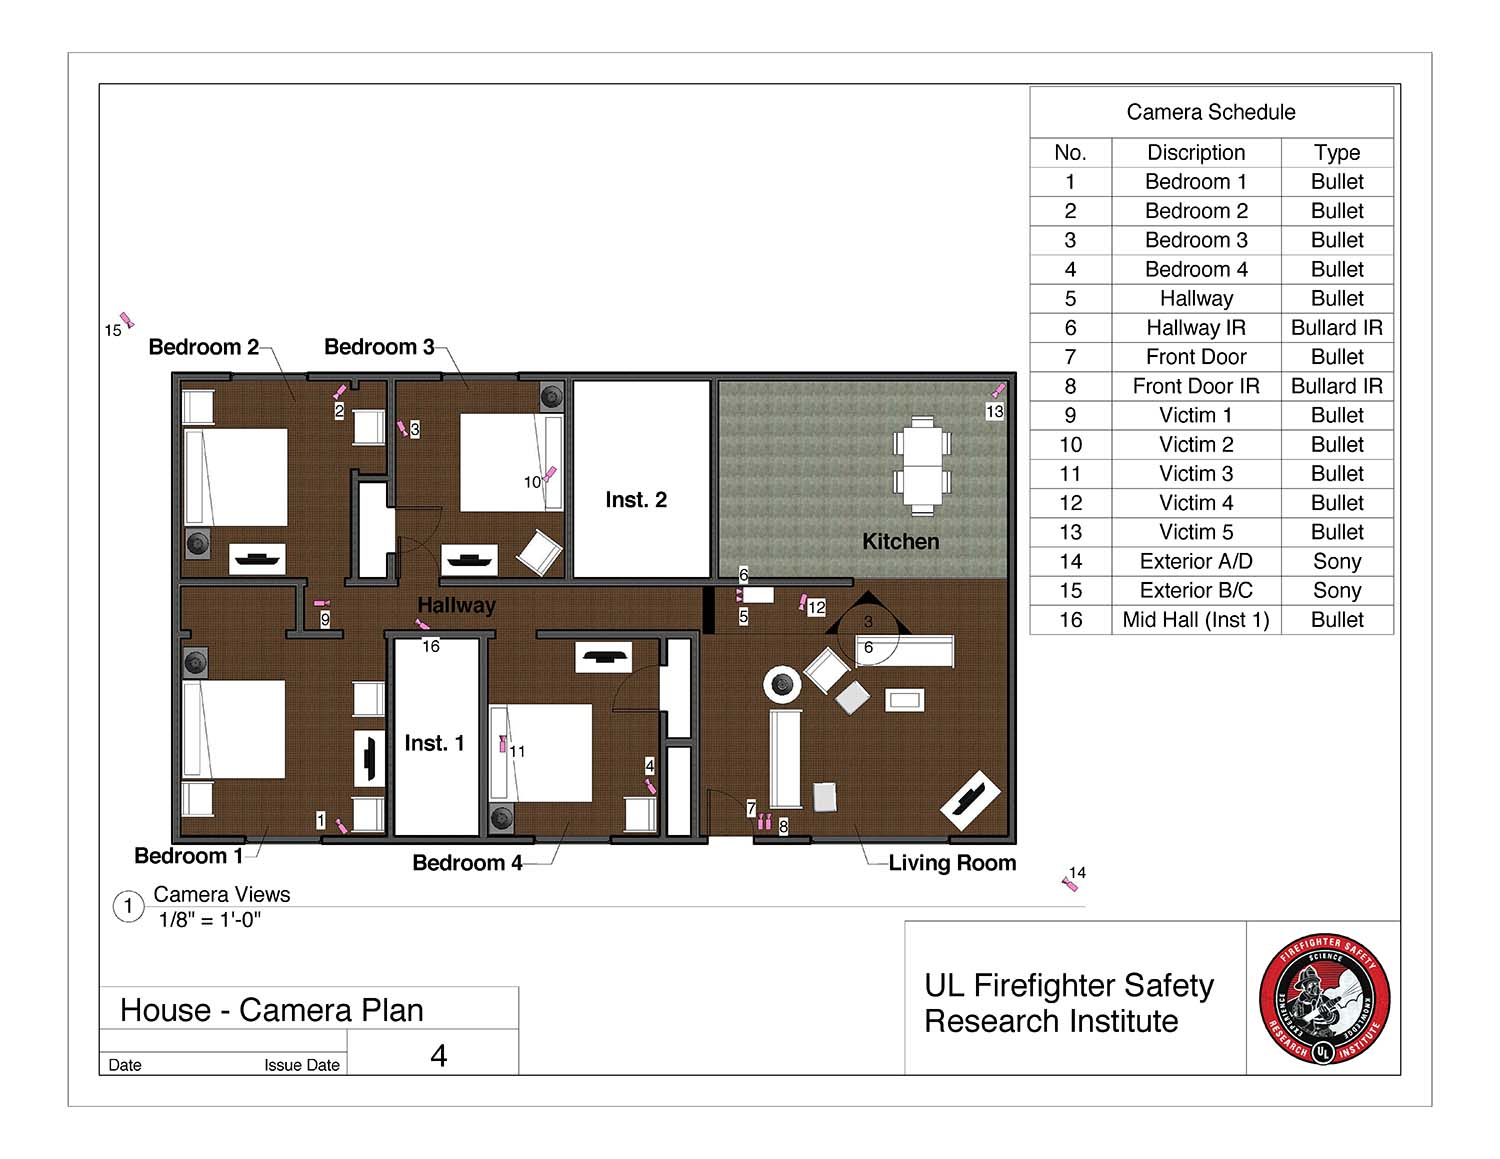
\includegraphics[width=\textheight]{../0_Images/Appendix_Figures/Camera_Plan}
\caption[]{Camera Plan}
\label{fig:appendix_cameras}
\end{sidewaysfigure}
